\documentclass[12pt,a4paper]{book}
\newcommand{\niveau}{4\textsuperscript{e}}
% ================================
% PRÉAMBULE COMMUN — Mathématiques (6e, 5e, 4e)
% ================================

% Encodage et langue
\usepackage[T1]{fontenc}
\usepackage[french]{babel}

% Typographie moderne
\usepackage{newtxtext,newtxmath}

% Configuration des pages
\usepackage{geometry}
\geometry{top=2.5cm, bottom=2.5cm, left=2.5cm, right=2.5cm}

% Amélioration du rendu
\usepackage{microtype}

% Personnalisation des titres
\usepackage{titlesec}
\titleformat{\chapter}[hang]{\huge\bfseries}{\thechapter.}{0.6em}{}
\titleformat{\section}[hang]{\Large\bfseries}{\thesection}{0.6em}{}
\titleformat{\subsection}[hang]{\large\bfseries}{\thesubsection}{0.6em}{}

% Ajustement de l'espacement des titres
\titlespacing{\chapter}{0pt}{-10pt}{20pt}
\titlespacing{\section}{0pt}{12pt}{8pt}
\titlespacing{\subsection}{0pt}{4pt}{2pt}

% En-têtes et pieds de page
\usepackage{fancyhdr}

% Packages mathématiques
\usepackage{amsmath, mathtools}
\usepackage{siunitx}

% Graphiques
\usepackage{tikz}
\usetikzlibrary{angles, quotes, calc, arrows.meta, shapes.geometric}
\usepackage{pgfplots}
\pgfplotsset{compat=1.18}

% Liens hypertexte
\usepackage{hyperref}
\hypersetup{
    colorlinks=true,
    linkcolor=blue!60!black,
    urlcolor=blue!60!black,
    citecolor=blue!60!black
}

% Boîtes colorées avec tcolorbox
\usepackage[most]{tcolorbox}

% Configuration globale des boîtes
\tcbset{
    rounded corners,
    boxsep=2ex,
    top=1.5ex,
    bottom=1.5ex,
    left=2.5ex,
    right=7ex,
    before skip=0pt,
    after skip=1.5ex,
    width=\textwidth,
    boxrule=1pt
}



% Définition des environnements personnalisés
\newtcolorbox{definitionbox}[1][]{
    colback=orange!5!white,
    colframe=orange!70!black,
    title={\textbf{Définition \thechapter.\number\numexpr\thedefinition+1\relax}\ifthenelse{\equal{#1}{}}{}{ : #1}},
    fonttitle=\bfseries,
    coltitle=black,
    before upper={\incdefinition}
}

\newtcolorbox{examplebox}{
    colback=green!5!white,
    colframe=green!60!black,
    title={\textbf{Exemple}},
    fonttitle=\bfseries,
    coltitle=black
}

\newtcolorbox{exercisebox}{
    colback=purple!5!white,
    colframe=purple!70!black,
    title={\textbf{Exercices}},
    fonttitle=\bfseries,
    coltitle=black
}

\newtcolorbox{objectifsbox}{
    colback=teal!5!white,
    colframe=teal!70!black,
    title={\textbf{Objectifs}},
    fonttitle=\bfseries,
    coltitle=black
}

\newtcolorbox{proprietebox}[1][]{
    colback=red!5!white,
    colframe=red!70!black,
    title={\textbf{Propriété \thechapter.\number\numexpr\thepropriete+1\relax}\ifthenelse{\equal{#1}{}}{}{ : #1}},
    fonttitle=\bfseries,
    coltitle=black,
    before upper={\incpropriete}
}

\newtcolorbox{activitybox}{
    colback=blue!5!white,
    colframe=blue!70!black,
    title={\textbf{Activité}},
    fonttitle=\bfseries,
    coltitle=black
}

\newtcolorbox{remarkbox}[1][]{
    colback=yellow!5!white,
    colframe=yellow!70!black,
    title={\textbf{Remarque \thechapter.\number\numexpr\theremarque+1\relax}\ifthenelse{\equal{#1}{}}{}{ : #1}},
    fonttitle=\bfseries,
    coltitle=black,
    before upper={\incremarque}
}

\newtcolorbox{quizbox}{
    colback=cyan!5!white,
    colframe=cyan!70!black,
    title={\textbf{Quiz}},
    fonttitle=\bfseries,
    coltitle=black
}

\newtcolorbox{methodebox}[1][]{
    colback=purple!5!white,
    colframe=purple!70!black,
    title={\textbf{Méthode \thechapter.\number\numexpr\themethode+1\relax}\ifthenelse{\equal{#1}{}}{}{ : #1}},
    fonttitle=\bfseries,
    coltitle=black,
    before upper={\incmethode}
}

% Compteurs pour les environnements (par chapitre)
\newcounter{definition}
\newcounter{propriete}
\newcounter{methode}
\newcounter{remarque}

% Réinitialisation des compteurs au début de chaque chapitre
\makeatletter
\@addtoreset{definition}{chapter}
\@addtoreset{propriete}{chapter}
\@addtoreset{methode}{chapter}
\@addtoreset{remarque}{chapter}
\makeatother

% Commandes pour incrémenter automatiquement les compteurs
\newcommand{\incdefinition}{\stepcounter{definition}}
\newcommand{\incpropriete}{\stepcounter{propriete}}
\newcommand{\incmethode}{\stepcounter{methode}}
\newcommand{\incremarque}{\stepcounter{remarque}}

% Commande personnalisée pour les trous
\newcommand{\trous}[1]{\makebox[#1]{\rule{0pt}{1.2ex}\dotfill}}

% Variable pour stocker le titre de la séquence
\newcommand{\seqtitle}{}
\newcommand{\setseqtitle}[1]{\renewcommand{\seqtitle}{#1}}

% Mise en page de l'en-tête et du pied
\pagestyle{fancy}
\setlength{\headheight}{16pt} % FIX: évite le warning fancyhdr
\fancyhf{}
\lhead{Mathématiques \niveau{} -- 2025--2026}
\rhead{Seq.~\thechapter~--~\seqtitle}
\cfoot{\thepage}

% Listes compactes
\usepackage{enumitem}
\setlist[itemize]{left=1.2em}
\setlist[enumerate]{left=1.5em}

% Configuration des labels personnalisés pour enumitem
\SetEnumitemKey{a}{label=\alph*)}
\SetEnumitemKey{1}{label=\arabic*)}

% Définition des styles de listes personnalisés
\newlist{exerciselist}{enumerate}{1}
\setlist[exerciselist]{label=\alph*)}

\newlist{quizlist}{enumerate}{1}
\setlist[quizlist]{label=\arabic*)}

% Packages pour tableaux et présentations
\usepackage{longtable}
\usepackage{array}
\usepackage{booktabs}


\title{Cours de Mathématiques — Classe de 4\textsuperscript{e}\\[0.4em]\large Année scolaire 2025–2026}
\author{Abdoullatuf Maoulida}
\date{\today}

\begin{document}
\maketitle
\tableofcontents
\cleardoublepage

%\part{Nombres et calculs}
% Séquence 1 : Les nombres relatifs
\setseqtitle{Les nombres relatifs}
\chapter{Les nombres relatifs}

\begin{objectifsbox}
À l'issue de la séquence, l'élève sera capable de :
\begin{itemize}
\item Représenter et comparer des nombres relatifs sur une droite graduée
\item Calculer la distance à zéro d'un nombre relatif
\item Additionner et soustraire des nombres relatifs
\item Multiplier et diviser des nombres relatifs en appliquant la règle des signes
\item Généraliser la règle des signes pour plusieurs facteurs
\item Identifier et utiliser les nombres inverses
\item Résoudre des problèmes utilisant les nombres relatifs
\item Calculer des expressions numériques avec enchaînements d'opérations
\end{itemize}
\end{objectifsbox}

\section{Introduction aux nombres relatifs}

Les nombres relatifs sont utilisés dans de nombreuses situations de la vie quotidienne :
\begin{itemize}[label = \textbullet]
\item Mesurer des températures (température positive ou négative)
\item Mesurer des altitudes (au-dessus ou en dessous du niveau de la mer)
\item Gérer des soldes bancaires (crédit ou dette)
\item Se repérer dans le temps (avant ou après un événement)
\end{itemize}

Ils nous permettent de décrire des quantités qui peuvent être positives (au-dessus de zéro) ou négatives (en dessous de zéro).

\section{Définition et représentation}

\begin{definitionbox}
Un \textbf{nombre relatif} est un nombre qui peut être positif, négatif ou nul.
\end{definitionbox}

\subsection{La droite graduée}

Un nombre relatif est repéré par son signe (+ ou -) et sa distance à zéro.

Sur une droite graduée, le point de référence est l'origine (0).

\begin{proprietebox}
\begin{itemize}[label = \textbullet]
\item Les nombres positifs sont à droite de 0.
\item Les nombres négatifs sont à gauche de 0.
\item Plus un nombre est à droite, plus il est grand.
\item Plus un nombre est à gauche, plus il est petit.
\end{itemize}
\end{proprietebox}

\begin{examplebox}
Sur la droite graduée ci-dessous, on peut voir que $-3 < -1 < 0 < 2 < 5$

\begin{center}
\begin{tikzpicture}[scale=0.8]
\draw[->] (-6,0) -- (6,0);
\foreach \x in {-5,-4,-3,-2,-1,0,1,2,3,4,5}
    \draw (\x,0.2) -- (\x,-0.2) node[below] {$\x$};
\draw[fill=black] (-3,0) circle (2pt);
\draw[fill=black] (-1,0) circle (2pt);
\draw[fill=black] (0,0) circle (2pt);
\draw[fill=black] (2,0) circle (2pt);
\draw[fill=black] (5,0) circle (2pt);
\end{tikzpicture}
\end{center}
\end{examplebox}

\subsection{Distance à zéro}

\begin{definitionbox}
La \textbf{distance à zéro} d'un nombre relatif est la distance qui le sépare de 0 sur la droite graduée. C'est un nombre \textbf{toujours positif}.
\end{definitionbox}

\begin{examplebox}
\begin{itemize}[label = \textbullet]
\item La distance à zéro de +6 est \trous{2cm}
\item La distance à zéro de -4,5 est \trous{2cm}
\item La distance à zéro de 0 est \trous{2cm}
\end{itemize}
\end{examplebox}

\subsection{Nombres opposés}

\begin{definitionbox}
Deux nombres sont \textbf{opposés} s'ils ont la \textbf{même distance à zéro} mais des \textbf{signes différents}. Leur somme est toujours égale à 0.
\end{definitionbox}

\begin{examplebox}
\begin{itemize}[label = \textbullet]
\item L'opposé de +7 est \trous{2cm}
\item L'opposé de -2,3 est \trous{2cm}
\item L'opposé de 0 est \trous{2cm}
\end{itemize}
\end{examplebox}

\section{Addition et soustraction}
\subsection{Addition de nombres relatifs}
\begin{proprietebox}
Pour \textbf{additionner deux nombres de MÊME SIGNE :}
\begin{itemize}[label = \textbullet]
\item On \textbf{garde le signe commun}.
\item On \textbf{additionne} leurs distances à zéro.
\end{itemize}
\end{proprietebox}

\begin{examplebox}
\begin{align*}
(+5) + (+9) &= \trous{2cm} \quad \text{(Le signe commun est +, et } 5 + 9 = 14\text{)} \\
(-7) + (-3) &= \trous{2cm} \quad \text{(Le signe commun est -, et } 7 + 3 = 10\text{)} \\
(-1,5) + (-4) &= \trous{2cm}
\end{align*}
\end{examplebox}

\begin{proprietebox}
Pour \textbf{additionner deux nombres de SIGNE DIFFÉRENT :}
\begin{itemize}[label = \textbullet]
\item On \textbf{garde le signe du nombre qui a la plus grande distance à zéro}.
\item On \textbf{soustrait} la plus petite distance à zéro de la plus grande.
\end{itemize}
\end{proprietebox}

\begin{examplebox}
\begin{align*}
(+8) + (-3) &= \trous{2cm} \quad \text{(8 > 3, donc on garde le signe + et } 8 - 3 = 5\text{)} \\
(-6) + (+9) &= \trous{2cm} \quad \text{(9 > 6, donc on garde le signe + et } 9 - 6 = 3\text{)} \\
(+2,5) + (-7) &= \trous{2cm} \quad \text{(7 > 2,5, donc on garde le signe - et } 7 - 2,5 = 4,5\text{)}
\end{align*}
\end{examplebox}

\subsection{Soustraction de nombres relatifs}

\begin{proprietebox}
\textbf{Soustraire un nombre relatif, c'est ajouter son opposé :}
$$a - b = a + (-b)$$
\end{proprietebox}

\begin{examplebox}
\begin{align*}
(+5) - (+3) &= \trous{2.5cm} = \trous{2cm} \\
(+4) - (-2) &= \trous{2.5cm} = \trous{2cm} \\
(-7) - (+1) &= \trous{2.5cm} = \trous{2cm} \\
(-3) - (-5) &= \trous{2.5cm} = \trous{2cm}
\end{align*}
\end{examplebox}

\section{Multiplication et division}

\subsection{Règle des signes}

\begin{proprietebox}
\textbf{Règle des signes pour la multiplication et la division :}
\begin{itemize}[label = \textbullet]
\item Le produit (ou quotient) de deux nombres de \textbf{même signe} est \textbf{positif}
\item Le produit (ou quotient) de deux nombres de \textbf{signes contraires} est \textbf{négatif}
\end{itemize}
\end{proprietebox}

\begin{examplebox}
\begin{minipage}[t]{0.48\textwidth}
\textbf{Multiplication :}
\begin{align*}
(+4) \times (+3) &= \trous{2cm} \\
(-5) \times (-2) &= \trous{2cm} \\
(+6) \times (-3) &= \trous{2cm} \\
(-7) \times (+4) &= \trous{2cm}
\end{align*}
\end{minipage}
\hfill
\begin{minipage}[t]{0.48\textwidth}
\textbf{Division :}
\begin{align*}
(+15) \div (+3) &= \trous{2cm} \\
(-20) \div (-4) &= \trous{2cm} \\
(+24) \div (-6) &= \trous{2cm} \\
(-35) \div (+7) &= \trous{2cm}
\end{align*}
\end{minipage}
\end{examplebox}

\subsection{Généralisation de la règle des signes}
\begin{proprietebox}
\textbf{Produit de plusieurs nombres relatifs :}
Le produit de plusieurs nombres relatifs sera de signe :
\begin{itemize}[label = \textbullet]
\item \textbf{positif} s'il y a un nombre \textbf{pair} de facteurs négatifs
\item \textbf{négatif} s'il y a un nombre \textbf{impair} de facteurs négatifs
\end{itemize}
\end{proprietebox}

\begin{examplebox}
\textbf{Déterminer le signe des produits suivants :}

\begin{align*}
A &= (-2) \times (+3) \times (-4) \times (-1) \\
B &= (-1) \times (-2) \times (-3) \times (-4) \\
C &= (+5) \times (-6) \times (+7) \times (-8) \times (-9)
\end{align*}

\begin{itemize}[label = \textbullet]
\item $A$ est \trous{2.5cm} car il y a \trous{1.5cm} facteurs négatifs et \trous{1.5cm} est un nombre impair.
\item $B$ est \trous{2.5cm} car il y a \trous{1.5cm} facteurs négatifs et \trous{1.5cm} est un nombre pair.
\item $C$ est \trous{2.5cm} car il y a \trous{1.5cm} facteurs négatifs et \trous{1.5cm} est un nombre impair.
\end{itemize}
\end{examplebox}

\subsection{Nombres inverses}
\begin{definitionbox}
Deux nombres relatifs sont des \textbf{nombres inverses} si leur produit est égal à 1.

Soit $a$ et $b$ deux nombres relatifs. $a$ et $b$ sont dits « inverses » si et seulement si $a \times b = 1$.
\end{definitionbox}

\begin{examplebox}
\begin{itemize}[label = \textbullet]
\item L'inverse de 5 est \trous{1cm} car $5 \times \trous{1cm} = 1$
\item L'inverse de $-\frac{2}{3}$ est \trous{1cm} car $-\frac{2}{3} \times$ \trous{1cm} = 1
\item L'inverse de -4 est \trous{1cm} car $-4 \times$ \trous{1cm} = 1
\end{itemize}
\end{examplebox}

\subsection{Simplification des écritures}
\begin{remarkbox}
\textbf{Conventions d'écriture :}
\begin{itemize}[label = \textbullet]
\item On peut écrire $+5$ au lieu de $(+5)$
\item On peut écrire $-3$ au lieu de $(-3)$
\item Le signe $+$ peut être omis pour les nombres positifs : $5$ au lieu de $+5$
\item Le signe $-$ ne peut jamais être omis pour les nombres négatifs
\end{itemize}
\end{remarkbox}

\section{Expressions numériques et enchaînements d'opérations}
\begin{methodebox}
\textbf{Pour calculer une expression numérique :}
\begin{enumerate}[label = \arabic*)]
\item On effectue en premier les calculs dans les \textbf{parenthèses les plus intérieures}
\item On calcule les \textbf{puissances} éventuelles
\item On effectue ensuite les \textbf{multiplications et divisions} avant les additions et soustractions
\item Si plusieurs multiplications/divisions se suivent, on calcule dans le \textbf{sens de la lecture}
\item Si plusieurs additions/soustractions se suivent, on calcule dans le \textbf{sens de la lecture}
\end{enumerate}
\end{methodebox}

\begin{examplebox}
\textbf{Calculer les expressions suivantes :}

\noindent
\begin{minipage}[t]{0.48\textwidth}
\begin{align*}
A &= 5 + 3 \times (-2) \\
  &= \trous{2.5cm} \\
  &= \trous{2.5cm}
\end{align*}
\end{minipage}
\hfill
\begin{minipage}[t]{0.48\textwidth}
\begin{align*}
B &= (-8) \div 2 + 3 \times (-1) \\
  &= \trous{2.5cm} \\
  &= \trous{2.5cm}
\end{align*}
\end{minipage}

\vspace{1em}

\noindent
\begin{minipage}[t]{0.48\textwidth}
\begin{align*}
C &= [(-6) + 4] \times (-2) \\
  &= \trous{2.5cm} \\
  &= \trous{2.5cm}
\end{align*}
\end{minipage}
\hfill
\begin{minipage}[t]{0.48\textwidth}
\begin{align*}
D &= 12 \div (-3) \times 2 \\
  &= \trous{2.5cm} \\
  &= \trous{2.5cm}
\end{align*}
\end{minipage}
\end{examplebox}

\section{Exercices d'application}

\begin{exercisebox}
\textbf{Exercice 1 :} Représenter et comparer

\begin{enumerate}[label=\alph*)]
\item Représenter sur une droite graduée les nombres : $-4$ ; $+2$ ; $-1$ ; $+5$ ; $0$ ; $-3$
\item Ranger ces nombres dans l'ordre croissant
\item Donner la distance à zéro de chaque nombre
\end{enumerate}

\textbf{Exercice 2 :} Calculs avec les nombres relatifs

Calculer les expressions suivantes :
\begin{enumerate}[label=\alph*)]
	\item $A = (+7) + (-3) + (+2)$
	\item $B = (-5) + (+8) + (-1)$
	\item $C = (+4) - (-6) + (-2)$
	\item $D = (-3) - (+5) - (-2)$
\end{enumerate}

\textbf{Exercice 3 :} Multiplication et division

Calculer :
\begin{enumerate}[label=\alph*)]
	\item $E = (+6) \times (-4)$
	\item $F = (-8) \times (-3)$
	\item $G = (+24) \div (-6)$
	\item $H = (-35) \div (-7)$
\end{enumerate}

\textbf{Exercice 4 :} Généralisation de la règle des signes

Déterminer le signe des produits suivants :
\begin{enumerate}[label=\alph*)]
	\item $I = (-2) \times (+3) \times (-4)$
	\item $J = (-1) \times (-2) \times (-3) \times (-4)$
	\item $K = (+5) \times (-6) \times (+7) \times (-8)$
\end{enumerate}

\textbf{Exercice 5 :} Expressions numériques

Calculer les expressions suivantes :
\begin{enumerate}[label=\alph*)]
	\item $L = 8 + 3 \times (-2)$
	\item $M = (-12) \div 3 + 2 \times (-1)$
	\item $N = [(-5) + 3] \times (-2)$
	\item $O = 15 \div (-3) \times 2$
\end{enumerate}

\textbf{Exercice 6 :} Problème

La température était de $-5\,\text{°C}$ le matin. Elle a augmenté de $+8\,\text{°C}$ dans la journée, puis baissé de $-3\,\text{°C}$ le soir.

\begin{enumerate}[label=\alph*)]
	\item Quelle était la température en fin de journée ?
	\item Quelle était la température le soir ?
\end{enumerate}
\end{exercisebox}

\begin{exercisebox}
\textbf{Exercice 7 :} Nombres inverses

Trouver l'inverse de chacun des nombres suivants :
\begin{enumerate}[label=\alph*)]
	\item $+6$
	\item $-\frac{1}{4}$
	\item $+2,5$
	\item $-\frac{3}{7}$
\end{enumerate}
\end{exercisebox}

 % Les nombres relatifs
% Chapitre 2 : Théorème de Pythagore et sa réciproque
% Version améliorée conforme à la réforme du collège 2025
\chapter{Théorème de Pythagore et sa réciproque}

\section{Introduction}
Le théorème de Pythagore est l'un des théorèmes les plus célèbres et les plus utiles de la géométrie. Il porte le nom de Pythagore, mathématicien et philosophe grec du VI\textsuperscript{e} siècle avant J.-C., bien que cette relation ait été découverte par plusieurs civilisations antérieures (Babyloniens, Égyptiens, Chinois).

Ce théorème établit une relation fondamentale entre les côtés d'un triangle rectangle et trouve de nombreuses applications dans la vie courante : architecture, navigation, cartographie, sport, etc.

\textbf{Problématique du chapitre :} Comment calculer des longueurs dans un triangle rectangle ? Comment déterminer si un triangle est rectangle ?

\section{Activité d'approche : découverte par manipulation}

\textbf{Objectif :} Découvrir la relation entre les aires des carrés construits sur les côtés d'un triangle rectangle.

\textbf{Matériel :} Papier quadrillé, ciseaux, règle graduée

\textbf{Consigne :}
\begin{enumerate}
    \item Construire plusieurs triangles rectangles sur papier quadrillé
    \item Construire un carré sur chacun des trois côtés
    \item Compter le nombre de carreaux (ou calculer l'aire) de chaque carré
    \item Chercher une relation entre ces trois nombres
\end{enumerate}

\textbf{Constat :} Pour tout triangle rectangle, l'aire du carré construit sur l'hypoténuse est égale à la somme des aires des carrés construits sur les deux autres côtés.

\section{Définitions et vocabulaire}

\begin{definitionbox}[Vocabulaire du triangle rectangle]
Un triangle ayant un angle droit est un triangle rectangle. Les deux côtés perpendiculaires d’un triangle rectangle sont les \textbf{côtés de l’angle droit}. Le côté restant est l’\textbf{hypoténuse} du triangle rectangle. C’est le \textbf{côté opposé} à l’angle droit.
\end{definitionbox}

\begin{proprietebox}[Hypoténuse]
	Si un triangle est rectangle alors son plus grand côté est l’hypoténuse. \qquad (Admise)
\end{proprietebox}

\section{Le théorème de Pythagore}

\subsection{Énoncé du théorème}

\begin{theoremebox}[Théorème de Pythagore]
Dans un triangle rectangle, le carré de la longueur de l'hypoténuse est égal à la somme des carrés des longueurs des deux autres côtés.

\textbf{Formulation mathématique :}\\
Si $ABC$ est un triangle rectangle en $A$, alors : $BC^2 = AB^2 + AC^2$ (\textbf{Égalité de Pythagore})

\begin{center}
	\begin{tikzpicture}[scale=1.2]
		% Triangle rectangle
		\coordinate (A) at (0,0);
		\coordinate (B) at (3,0);
		\coordinate (C) at (0,2);
		
		% Tracé du triangle
		\draw[thick] (A) -- (B) -- (C) -- cycle;
		
		% Angle droit
		\draw (0.3,0) -- (0.3,0.3) -- (0,0.3);
		
		% Étiquettes
		\node[below left] at (A) {$A$};
		\node[below right] at (B) {$B$};
		\node[above left] at (C) {$C$};
		
		% Côtés
		\node[below] at (1.5,0) {$c$};
		\node[left] at (0,1) {$b$};
		\node[above right] at (1.5,1) {$a$ (hypoténuse)};
	\end{tikzpicture}
\end{center}
\end{theoremebox}

\subsection{Démonstration du théorème de Pythagore par la méthode des aires}
Considérons un carré de côté $(a + b)$ contenant quatre triangles rectangles identiques de côtés $a$, $b$ et d'hypoténuse $c$.

\begin{figure}[h]
\centering
\begin{minipage}{0.45\textwidth}
    \centering
    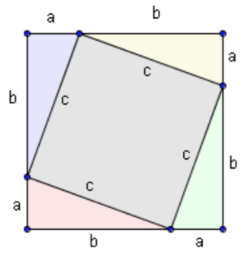
\includegraphics[width=0.8\textwidth]{../../assets/images/4e/seq_02_pythagore/fig_demo_pythagore_config_1}
    \caption{Configuration 1}
    \label{fig:config1}
\end{minipage}
\hfill
\begin{minipage}{0.45\textwidth}
    \centering
    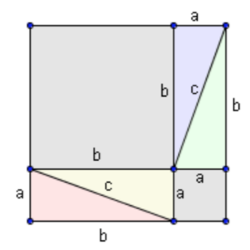
\includegraphics[width=0.8\textwidth]{../../assets/images/4e/seq_02_pythagore/fig_demo_pythagore_config_2.png}
    \caption{Configuration 2}
    \label{fig:config2}
\end{minipage}
\end{figure}

\textbf{Configuration 1 :} Aire 1 = $(a+b)^2 = 4 \times \frac{ab}{2} + c^2 = 2ab + c^2$

\textbf{Configuration 2 :} Aire 2 = $(a+b)^2 = 4 \times \frac{ab}{2} + a^2 + b^2 = 2ab + a^2 + b^2$

Comme l'aire est la même dans les deux configurations (Aire 1 = Aire 2) :
$$2ab + c^2 = 2ab + a^2 + b^2 \Leftrightarrow c^2 = a^2 + b^2$$ \\
Ce qui démontre le théorème de Pythagore.

\section{Applications du théorème de Pythagore}

\subsection{Calculer la longueur de l'hypoténuse}

\begin{remarkbox}[Important]
$a^2 = a\times a$. À ne pas confondre avec $a \times 2 = a + a = 2a$
\end{remarkbox}

%\begin{methodebox}[Calculer la longueur de l'hypoténuse]
%Pour calculer la longueur de l'hypoténuse d'un triangle rectangle :
%\begin{enumerate}
%    \item Identifier le triangle rectangle et ses côtés
%    \item Repérer l'hypoténuse (côté opposé à l'angle droit)
%    \item Appliquer la formule : hypoténuse$^2$ = côté$_1^2$ + côté$_2^2$
%    \item Calculer la racine carrée du résultat
%\end{enumerate}
%\end{methodebox}

\begin{examplebox}
On étudie le triangle RAK rectangle en K tel que KR = 4,95 cm et KA= 6,6 cm. Calculons la mesure du côté [AR].

\noindent
\begin{minipage}[c]{0.60\textwidth}
Dans le triangle $RAK$ rectangle en $K$, d'après le théorème de Pythagore on a :
\begin{align*}
.........  &= .......... + .........\\
.........  &= .......... + ......... \\
.........  &= .......... + ......... \\
AR^2 &= ...........
\end{align*}
\end{minipage}
\hfill
\begin{minipage}[c]{0.35\textwidth}
	\centering
	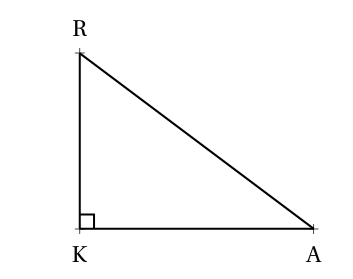
\includegraphics[width=\textwidth]{../../assets/images/4e/seq_02_pythagore/triangle_RKA_rectangle_en_K}
\end{minipage}

\vspace{1em}

\begin{minipage}[t]{\textwidth}
\textbf{Comment trouver $AR$ ?}

On ne connaît pas immédiatement un nombre dont le carré vaut exactement 68,0625.

Notons $x$ ce nombre. Comme $8^2 = 64 < 68,0625 < 81 = 9^2$, on en déduit que $8 < x < 9$.

En utilisant la calculatrice, on trouve que $8,2^2 = 67,24 < 68,0625 < 68,89 = 8,3^2$ et donc que $8,2 < x < 8,3$.

On constate alors que $8,25^2 = 68,0625$.

Finalement $AR = 8,25$ cm.
\end{minipage}
\end{examplebox}

\begin{proprietebox}[La racine carrée]
Pour tout nombre positif $a$, il existe un unique nombre \textbf{positif} dont le carré vaut exactement le nombre $a$.

Ce nombre s'appelle la \textbf{racine carrée} de $a$ et se note $\sqrt{a}$.

Par définition : $(\sqrt{a})^2 = \sqrt{a} \times \sqrt{a} = a$
\end{proprietebox}

\begin{examplebox}[Carrés parfaits]
\textbf{Quelques carrés parfaits à connaître :}

\begin{center}
\begin{tabular}{|c|c|c|c|c|c|c|c|c|c|c|c|c|c|}
\hline
$a$ & 0 & 1 & 2 & 3 & 4 & 5 & 6 & 7 & 8 & 9 & 10 & 11 & 12 \\
\hline
$a^2$ & ..... & ..... & ..... & ..... & ..... & ..... & ..... & ..... & ..... & ..... & ..... & ..... & ..... \\
\hline
\end{tabular}
\end{center}

Donc $\sqrt{0} = \trous{1.5cm}$ ; $\sqrt{1} = \trous{1.5cm}$ ; $\sqrt{9} = \trous{1.5cm}$ ; $\sqrt{16} = \trous{1.5cm}$ ; $\sqrt{25} = \trous{1.5cm}$ ; $\sqrt{36} = \trous{1.5cm}$ ; $\sqrt{49} = \trous{1.5cm}$ ; $\sqrt{64} = \trous{1.5cm}$ ;\\ $\sqrt{81} = \trous{1.5cm}$ ; $\sqrt{100} = \trous{1.5cm}$ ; $\sqrt{121} = \trous{1.5cm}$ ; $\sqrt{144} = \trous{1.5cm}$
\end{examplebox}


\subsection{Calculer la longueur d'un côté de l'angle droit}
\begin{methodebox}[Calculer la longueur d'un côté de l'angle droit]
Pour calculer la longueur d'un côté de l'angle droit :
\begin{enumerate}
    \item Identifier la longueur de l'hypoténuse et celle de l'autre côté de l'angle droit
    \item Appliquer la formule : hypoténuse$^2$ = côté$_1^2$ + côté$_2^2$
    \item Isoler le côté inconnu : côté$^2$ = hypoténuse$^2$ - autre côté$^2$
    \item Calculer la racine carrée du résultat
\end{enumerate}
\end{methodebox}

\begin{examplebox}
Un triangle $DEF$ est rectangle en $D$. $DE = 5$ cm et $EF = 13$ cm.\\
Calculer $DF$.

\textbf{Solution :}
\begin{itemize}
    \item Le triangle est rectangle en $D$, donc \trous{1.5cm} est l'hypoténuse.
    \item D'après le théorème de Pythagore : ....... = ........ + .......
    \item ....... = ........ + .......
    \item ....... = ........ + .......
    \item ....... = ........ + .......
    \item DF = ........... = ..........cm
\end{itemize}
\end{examplebox}

\section{La réciproque du théorème de Pythagore}

\subsection{Énoncé de la réciproque}
\begin{theoremebox}[Contra-posée du théorème de Pythagore]
	\textbf{Si} dans un triangle l’égalité de Pythagore n’est pas vérifiée \textbf{alors} ce triangle n’est pas rectangle. \qquad (\textit{Admise})
\end{theoremebox}
\begin{demobox}[Contra-posée du théorème de Pythagore]
C’est une conséquence de la logique des propositions.\\
Prenons un exemple simple :\\

\textbf{Propriété :} Si nous sommes le 25 décembre alors je ne vais pas à l’école. La propriété contra-posée est : Si je vais à l'école alors nous ne sommes pas le 25 décembre. On comprend que quand une propriété est vraie alors la propriété contra-posée est également vraie. Dans le cas du théorème de Pythagore, si l’égalité de Pythagore n’est pas vérifiée alors le triangle n’est pas rectangle car s’il était rectangle l’égalité serait vérifiée!
\end{demobox}
\begin{theoremebox}[Réciproque du théorème de Pythagore]
Si, dans un triangle, le carré de la longueur du plus grand côté est égal à la somme des carrés des longueurs des deux autres côtés, alors ce triangle est rectangle.
\end{theoremebox}


\subsection{Utilisation de la réciproque}
\begin{methodebox}[Démontrer qu'un triangle est rectangle]
Pour démontrer qu'un triangle est rectangle :
\begin{enumerate}
    \item Identifier le plus grand côté du triangle
    \item Calculer le carré de sa longueur
    \item Calculer la somme des carrés des deux autres côtés
    \item Comparer les résultats :
    \begin{itemize}
        \item Si égalité : le triangle est rectangle
        \item Si inégalité : le triangle n'est pas rectangle
    \end{itemize}
\end{enumerate}
\end{methodebox}

\begin{examplebox}
Un triangle a pour côtés 9 cm, 12 cm et 15 cm. Est-il rectangle ?

\textbf{Solution :}
\begin{itemize}
    \item Le plus grand côté mesure 15 cm
    \item $15^2 = ........$
    \item $9^2 + 12^2 = ........ + ......... = .........$
    \item Puisque .......... = ......... + .........., le triangle est rectangle
    \item L'angle droit est opposé au côté de 15 cm
\end{itemize}
\end{examplebox}

\begin{examplebox}
Un triangle a pour côtés 7 cm, 8 cm et 10 cm. Est-il rectangle ?

\textbf{Solution :}
\begin{itemize}
    \item Le plus grand côté mesure 10 cm
    \item $10^2 = .........$
    \item $7^2 + 8^2 = .......... + ......... = ..........$
    \item Puisque ........... $\neq$ ..........., le triangle .......................................
\end{itemize}
\end{examplebox}

\section{Applications et résolution de problèmes}

\subsection{Problèmes de la vie courante}

\begin{exercisebox}
\textbf{Exercice 1: L'échelle}\\

Une échelle de 4 m est appuyée contre un mur. Son pied est à 1,5 m du mur. À quelle hauteur le sommet de l'échelle touche-t-il le mur ?

\textbf{Solution :}

\begin{itemize}
    \item Triangle rectangle : mur, sol, échelle
    \item Hypoténuse : échelle = 4 m
    \item Un côté : distance au mur = 1,5 m
    \item Autre côté : hauteur = ?
\end{itemize}

$h^2 + 1,5^2 = 4^2$\\
$h^2 + 2,25 = 16$\\
$h^2 = 13,75$\\
$h = \sqrt{13,75} \approx 3,7$ m
\\

\textbf{Exercice 2: Vérification d'équerrage}\\

Un maçon vérifie qu'un angle est droit en mesurant les côtés d'un triangle formé par deux murs et une diagonale. Il mesure : 3 m, 4 m et 5 m. L'angle est-il droit ?

\textbf{Solution :}
\begin{itemize}
	\item Plus grand côté : 5 m
	\item $5^2 = 25$
	\item $3^2 + 4^2 = 9 + 16 = 25$
	\item Égalité vérifiée $\Rightarrow$ l'angle est droit
\end{itemize}
\end{exercisebox}

\subsection{Utilisation de la calculatrice}

\textbf{Compétence :} Utiliser la touche $\sqrt{}$ (racine carrée) de la calculatrice.

\textbf{Exemple :} Calculer $\sqrt{75}$
\begin{itemize}
    \item $\sqrt{75} = \sqrt{25 \times 3} = \sqrt{25} \times \sqrt{3} = 5\sqrt{3} \approx 8,66$
\end{itemize}

\subsection{Calculs exacts et valeurs approchées}

\textbf{Calcul exact :} $\sqrt{50} = \sqrt{25 \times 2} = 5\sqrt{2}$ cm\\
\textbf{Valeur approchée :} $\sqrt{50} \approx 7,07$ cm (arrondi au centième)



\section{Exercices d'application}

\subsection{Exercices de base}

\begin{exercisebox}
\textbf{Exercice 1:} Calculs directs :
\begin{enumerate}[label=\alph*)]
    \item Triangle rectangle : côtés 3 cm et 4 cm. Calculer l'hypoténuse.
    \item Triangle rectangle : hypoténuse 10 cm, un côté 6 cm. Calculer l'autre côté.
\end{enumerate}

\textbf{Exercice 2:}
Réciproque : Les triangles suivants sont-ils rectangles ?
\begin{enumerate}[label=\alph*)]
	\item Côtés : 7 cm, 24 cm, 25 cm
	\item Côtés : 6 cm, 7 cm, 8 cm
\end{enumerate}
\end{exercisebox}

\subsection{Exercices d'approfondissement}

\begin{exercisebox}
\textbf{Exercice 3:}
\textbf{Problème du terrain}\\
Un terrain rectangulaire mesure 40 m sur 30 m. Calculer la longueur de sa diagonale.

\textbf{Exercice 4:}
\textbf{Navigation}\\
Un bateau part d'un port et navigue 12 km vers l'est puis 5 km vers le nord. À quelle distance se trouve-t-il du port ?

\textbf{Exercice 5:}
\textbf{Architecture}\\
Pour vérifier qu'un mur est perpendiculaire au sol, un architecte place un point A sur le mur à 3 m du sol, un point B au pied du mur, et un point C sur le sol à 4 m de B. Si AC = 5 m, le mur est-il perpendiculaire au sol ?
\end{exercisebox}

\section{Activité TICE}

\subsection{Utilisation d'un logiciel de géométrie dynamique}

\textbf{Objectif :} Vérifier le théorème de Pythagore avec GeoGebra

\textbf{Consignes :}
\begin{enumerate}
    \item Construire un triangle rectangle ABC
    \item Construire les carrés sur chaque côté
    \item Afficher les aires des trois carrés
    \item Modifier la forme du triangle et observer
    \item Conjecture sur la relation entre ces aires
\end{enumerate}

%\section{Liens avec d'autres notions mathématiques}
%
%\subsection{Distance entre deux points dans un repère}
%
%Le théorème de Pythagore permet de calculer la distance entre deux points dans un repère orthonormé.
%
%Si $A(x_A, y_A)$ et $B(x_B, y_B)$ sont deux points dans un repère orthonormé, alors la distance $AB$ est donnée par :
%\[AB = \sqrt{(x_B - x_A)^2 + (y_B - y_A)^2}\]
%
%\begin{examplebox}
%Calculons la distance entre les points $A(2, 3)$ et $B(6, 7)$ dans un repère orthonormé.
%
%En appliquant le théorème de Pythagore :
%\[AB^2 = (6-2)^2 + (7-3)^2 = 4^2 + 4^2 = 16 + 16 = 32\]
%\[AB = \sqrt{32} = \sqrt{16 \times 2} = 4\sqrt{2}\]
%
%La distance entre $A$ et $B$ est $4\sqrt{2}$ unités.
%\end{examplebox}
%
%\subsection{Équations et théorème de Pythagore}
%
%Le théorème de Pythagore conduit souvent à des équations qu'il faut résoudre pour trouver des longueurs.
%
%\begin{examplebox}
%Dans un triangle rectangle $ABC$ rectangle en $A$, on sait que $AB = x$ cm, $AC = (x+3)$ cm et $BC = 17$ cm. Déterminons la valeur de $x$.
%
%D'après le théorème de Pythagore :
%\[BC^2 = AB^2 + AC^2\]
%\[17^2 = x^2 + (x+3)^2\]
%\[289 = x^2 + x^2 + 6x + 9\]
%\[289 = 2x^2 + 6x + 9\]
%\[2x^2 + 6x - 280 = 0\]
%\[x^2 + 3x - 140 = 0\]
%
%En factorisant : $(x - 10)(x + 14) = 0$
%
%Les solutions sont $x = 10$ et $x = -14$.
%
%Comme une longueur ne peut pas être négative, nous avons $x = 10$ cm.
%
%Donc $AB = 10$ cm et $AC = 13$ cm.
%\end{examplebox}
%
%\section{Pour aller plus loin}
%
%\subsection{Histoire des mathématiques}
%\begin{itemize}
%    \item Les tablettes babyloniennes (Plimpton 322)
%    \item La démonstration par le président Garfield
%    \item Les différentes démonstrations du théorème (plus de 300 connues)
%\end{itemize}
%
%\subsection{Généralisation}
%\begin{itemize}
%    \item Théorème de Pythagore généralisé (loi des cosinus)
%    \item Théorème de Pythagore dans l'espace à n dimensions
%\end{itemize}
%
%\subsection{Applications modernes}
%\begin{itemize}
%    \item GPS et géolocalisation
%    \item Graphisme 3D et jeux vidéo
%    \item Architecture et ingénierie
%\end{itemize}

\section{Synthèse du chapitre}

\textbf{Ce qu'il faut retenir :}

\begin{enumerate}
    \item \textbf{Théorème de Pythagore :} Dans un triangle rectangle, hypoténuse$^2$ = côté$_1^2$ + côté$_2^2$
    \item \textbf{Réciproque :} Si dans un triangle, le carré du plus grand côté égale la somme des carrés des deux autres, alors le triangle est rectangle
    \item \textbf{Applications :} Calcul de longueurs, vérification d'angles droits, résolution de problèmes concrets
    \item \textbf{Méthodes :} Identification du triangle rectangle, application des formules, utilisation de la calculatrice
\end{enumerate}

\textbf{Liens avec d'autres chapitres :}
\begin{itemize}
    \item Racines carrées (chapitre précédent)
    \item Trigonométrie (chapitre à venir)
    \item Géométrie dans l'espace
    \item Fonctions (distance entre deux points dans un repère)
\end{itemize}  % Théorème de Pythagore
%\chapter{Fractions décimales et nombres décimaux}
\label{chap:seq03}

\begin{definitionbox}
\textbf{Objectifs d'apprentissage.} À l'issue de la séquence, l'élève sera capable de :
\begin{itemize}
  \item ...
\end{itemize}
\end{definitionbox}

\section*{Pré-requis}
\begin{itemize}
  \item ...
\end{itemize}

\section{Découverte}
\begin{examplebox}
Problème d'introduction ou situation de découverte.
\end{examplebox}

\section{Leçon}
\begin{itemize}
  \item Rappels et définitions.
  \item Méthodes et exemples guidés.
\end{itemize}

\section{Exercices d'entraînement}
\begin{exercisebox}
Exercice 1.
\end{exercisebox}

\begin{exercisebox}
Exercice 2.
\end{exercisebox}

\section{Évaluation rapide (5 à 10 min)}
\begin{exercisebox}
Mini-quiz.
\end{exercisebox}
 % Équations
%\input{chapitres/seq_04} % Proportionnalité
%% Séquence 5 : Notion de proportionnalité
\setseqtitle{Notion de proportionnalité}
\chapter{Notion de proportionnalité}
\label{chap:seq05}

\begin{definitionbox}
\textbf{Objectifs d'apprentissage.} À l'issue de la séquence, l'élève sera capable de :
\begin{itemize}
  \item ...
\end{itemize}
\end{definitionbox}

\section*{Pré-requis}
\begin{itemize}
  \item ...
\end{itemize}

\section{Découverte}
\begin{examplebox}
Problème d'introduction ou situation de découverte.
\end{examplebox}

\section{Leçon}
\begin{itemize}
  \item Rappels et définitions.
  \item Méthodes et exemples guidés.
\end{itemize}

\section{Exercices d'entraînement}
\begin{exercisebox}
Exercice 1.
\end{exercisebox}

\begin{exercisebox}
Exercice 2.
\end{exercisebox}

\section{Évaluation rapide (5 à 10 min)}
\begin{exercisebox}
Mini-quiz.
\end{exercisebox}
 % Statistiques
%% Séquence 6 : Notion de probabilités
\chapter{Notion de probabilités}
\label{chap:seq06}

\begin{definitionbox}
\textbf{Objectifs d'apprentissage.} À l'issue de la séquence, l'élève sera capable de :
\begin{itemize}
  \item ...
\end{itemize}
\end{definitionbox}

\section*{Pré-requis}
\begin{itemize}
  \item ...
\end{itemize}

\section{Découverte}
\begin{examplebox}
Problème d'introduction ou situation de découverte.
\end{examplebox}

\section{Leçon}
\begin{itemize}
  \item Rappels et définitions.
  \item Méthodes et exemples guidés.
\end{itemize}

\section{Exercices d'entraînement}
\begin{exercisebox}
Exercice 1.
\end{exercisebox}

\begin{exercisebox}
Exercice 2.
\end{exercisebox}

\section{Évaluation rapide (5 à 10 min)}
\begin{exercisebox}
Mini-quiz.
\end{exercisebox}
 % Géométrie dans l'espace
%% Séquence 7 : Angles et rapporteur
\chapter{Angles et rapporteur}
\label{chap:seq07}

\begin{definitionbox}
\textbf{Objectifs d'apprentissage.} À l'issue de la séquence, l'élève sera capable de :
\begin{itemize}
  \item ...
\end{itemize}
\end{definitionbox}

\section*{Pré-requis}
\begin{itemize}
  \item ...
\end{itemize}

\section{Découverte}
\begin{examplebox}
Problème d'introduction ou situation de découverte.
\end{examplebox}

\section{Leçon}
\begin{itemize}
  \item Rappels et définitions.
  \item Méthodes et exemples guidés.
\end{itemize}

\section{Exercices d'entraînement}
\begin{exercisebox}
Exercice 1.
\end{exercisebox}

\begin{exercisebox}
Exercice 2.
\end{exercisebox}

\section{Évaluation rapide (5 à 10 min)}
\begin{exercisebox}
Mini-quiz.
\end{exercisebox}
 % Théorème de Pythagore
%\setseqtitle{Opérations avec les nombres décimaux}
\chapter{Opérations avec les nombres décimaux}
\label{chap:seq08}

\begin{objectifsbox}
\textbf{Objectifs d'apprentissage.} À l'issue de la séquence, l'élève sera capable de :
\begin{itemize}
  \item Additionner et soustraire des nombres décimaux
  \item Multiplier des nombres décimaux
  \item Poser correctement les opérations avec des nombres décimaux
  \item Calculer des ordres de grandeur
\end{itemize}
\end{objectifsbox}

\section*{Pré-requis}
\begin{itemize}
  \item Connaissance des nombres entiers et de leurs opérations
  \item Maîtrise de la numération décimale
  \item Compréhension de la valeur des chiffres selon leur position
\end{itemize}

\section{Addition et soustraction avec des nombres décimaux}

\begin{definitionbox}
	\textbf{Addition et soustraction}
	
	On calcule une \textbf{\trous{3cm}} lorsqu'on ajoute deux nombres, et une \textbf{\trous{3cm}} lorsqu'on en soustrait deux.
	
	Le résultat d'une addition est une \textbf{\trous{2.5cm}}, celui d'une soustraction une \textbf{\trous{2.5cm}}.
	
	Les nombres calculés ensemble s'appellent les \textbf{\trous{2.5cm}}.
\end{definitionbox}

\begin{examplebox}
	\begin{center}
		\begin{tabular}{p{0.45\textwidth}p{0.45\textwidth}}
			\textbf{21,5 + 12,3 = 33,8} (\trous{2.5cm}) & \textbf{21,5 - 12,3 = 9,2} (\trous{2.5cm}) \\
			On dit que << 33,8 est la somme de 21,5 et 12,3 >> & On dit que << 9,2 est la différence de 21,5 par 12,3 >> \\
		\end{tabular}
	\end{center}
	
	Dans les deux cas, les deux nombres \textbf{21,5} et \textbf{12,3} sont les \textbf{termes} du calcul.
\end{examplebox}

\begin{proprietebox}
On peut échanger les termes d'une addition sans modifier son résultat. On dit que l'addition est \textbf{\trous{3cm}}.
\end{proprietebox}

\textbf{ATTENTION :} Ce n'est pas vrai pour une soustraction !

% Exemple 1 : opération en ligne dans une boxe
\begin{examplebox}
	\begin{center}
		\begin{tabular}{p{0.45\textwidth} p{0.45\textwidth}}
			\textbf{Exemple 1 (opération en ligne)} : \\
			$8,5 + 7,2 + 2,1 + 3,4$ & $8,5 - 3,2$ \\
			$= \underline{\trous{1cm} + \trous{1cm}} + \underline{\trous{1cm} + \trous{1cm}}$ & $= 5,3$ \\
			$= 10,6 + 10,6$ & (attention : on ne sait pas encore calculer $3,2 - 8,5$) \\
			$= 21,2$ & \\
		\end{tabular}
	\end{center}
\end{examplebox}

\vspace{0.5cm}

% Exemple 2 : opération posée dans une boxe
\begin{examplebox}
	\begin{center}
		\begin{tabular}{p{0.45\textwidth} p{0.45\textwidth}}
			\textbf{Exemple 2 (opération posée)} : \underline{\textbf{28,4 + 84,39}} 
			& 
			\underline{\textbf{20,18 - 19,45}} \\
			
			\begin{tabular}{r}
				84,39 \\
				+ 28,40 \\
				\hline
				\trous{1.5cm}
			\end{tabular} &
			\begin{tabular}{r}
				20,18 \\
				- 19,45 \\
				\hline
				\trous{1.5cm}
			\end{tabular} \\
			
		\end{tabular}
	\end{center}
\end{examplebox}


\textbf{Remarques :}
\begin{itemize}
	\item Les mots << \textbf{addition} >> et << \textbf{soustraction} >> désignent des opérations, tandis que les mots << \textbf{somme} >> et << \textbf{différence} >> désignent des nombres (des résultats).
	\item Pour poser une addition ou une soustraction de nombres décimaux, il faut impérativement aligner les nombres par la droite et aligner les virgules.
	\item On peut ajouter des zéros à droite d'un nombre décimal sans changer sa valeur (exemple : 28,4 = 28,40).
\end{itemize}

\section{Multiplication avec des nombres décimaux}

\begin{definitionbox}
	\textbf{Multiplication}
	
	Dans une \textbf{multiplication}, on multiplie des \trous{2.5cm}, et le résultat est un \trous{2cm}.
\end{definitionbox}

\begin{examplebox}
	On dit que 60,5 est le \trous{2.5cm} de 12,1 par 5
\end{examplebox}

\begin{proprietebox}
On peut échanger l'ordre des facteurs sans changer le résultat. On dit que la multiplication est \trous{3cm}.
\end{proprietebox}

\textbf{Méthode :} Poser une multiplication avec des nombres décimaux.

\textbf{Exemple :} $25,1 \times 7,53$

\begin{center}
	\begin{tabular}{r}
		25,1 \\
		$\times$ 7,53 \\
		\hline
		\trous{2cm} \\
		\trous{2cm} \\
		\trous{2cm} \\
		\hline
		\trous{2cm}
	\end{tabular}
\end{center}

\textbf{Règle pour placer la virgule :} Le nombre de chiffres après la virgule dans le résultat est égal à la somme du nombre de chiffres après la virgule dans chaque facteur.

\section{Ordre de grandeur}

\begin{definitionbox}
	\textbf{Ordre de grandeur}
	
	Un \textbf{ordre de grandeur} d'un nombre est un nombre proche de celui-ci et facile à utiliser en calcul mental.
	
	\textbf{Remarque :} Un ordre de grandeur n'est pas unique : on peut donner des ordres de grandeur différents selon la précision voulue.
\end{definitionbox}

\begin{examplebox}
	La population française était de 67 063 703 habitants en 2020. Un ordre de grandeur de cette population est \trous{3cm} (on pourrait aussi choisir 100 millions ou 67 millions).
\end{examplebox}

\begin{examplebox}
Pour calculer $24,7 \times 3,8$, on peut d'abord estimer :

• 24,7 $\approx$ 25 (ordre de grandeur)

• 3,8 $\approx$ 4 (ordre de grandeur)

• Donc $24,7 \times 3,8 \approx 25 \times 4 = 100$

Le résultat exact sera proche de 100.
\end{examplebox}

\section{Exercices d'entraînement}

\begin{exercisebox}
\textbf{Exercices d'application :} Pose et calcule les opérations suivantes :
\begin{enumerate}
	\item 45,7 + 23,8
	\item 67,2 - 34,5
	\item $12,3 \times 4,6$
\end{enumerate}
\end{exercisebox}

\begin{exercisebox}
\textbf{Exercices d'application :} Donne un ordre de grandeur de chaque calcul, puis calcule le résultat exact :
\begin{enumerate}
	\item 23,4 + 45,7
	\item 89,2 - 12,8
	\item $15,6 \times 3,2$
\end{enumerate}
\end{exercisebox}

\section{Évaluation rapide (5 à 10 min)}

\begin{exercisebox}
\textbf{Évaluation rapide :}
\begin{enumerate}
	\item Quel est le résultat de 12,5 + 8,7 ?
	\item Calcule 45,2 - 23,8
	\item Donne un ordre de grandeur de $34,7 \times 2,1$
\end{enumerate}
\end{exercisebox}
 % Théorème de Thalès
%\chapter{La médiatrice d’un segment}
\label{chap:seq09}

\begin{definitionbox}
\textbf{Objectifs d'apprentissage.} À l'issue de la séquence, l'élève sera capable de :
\begin{itemize}
  \item ...
\end{itemize}
\end{definitionbox}

\section*{Pré-requis}
\begin{itemize}
  \item ...
\end{itemize}

\section{Découverte}
\begin{examplebox}
Problème d'introduction ou situation de découverte.
\end{examplebox}

\section{Leçon}
\begin{itemize}
  \item Rappels et définitions.
  \item Méthodes et exemples guidés.
\end{itemize}

\section{Exercices d'entraînement}
\begin{exercisebox}
Exercice 1.
\end{exercisebox}

\begin{exercisebox}
Exercice 2.
\end{exercisebox}

\section{Évaluation rapide (5 à 10 min)}
\begin{exercisebox}
Mini-quiz.
\end{exercisebox}
 % Trigonométrie
%\chapter{La division}
\label{chap:seq10}

\begin{definitionbox}
\textbf{Objectifs d'apprentissage.} À l'issue de la séquence, l'élève sera capable de :
\begin{itemize}
  \item ...
\end{itemize}
\end{definitionbox}

\section*{Pré-requis}
\begin{itemize}
  \item ...
\end{itemize}

\section{Découverte}
\begin{examplebox}
Problème d'introduction ou situation de découverte.
\end{examplebox}

\section{Leçon}
\begin{itemize}
  \item Rappels et définitions.
  \item Méthodes et exemples guidés.
\end{itemize}

\section{Exercices d'entraînement}
\begin{exercisebox}
Exercice 1.
\end{exercisebox}

\begin{exercisebox}
Exercice 2.
\end{exercisebox}

\section{Évaluation rapide (5 à 10 min)}
\begin{exercisebox}
Mini-quiz.
\end{exercisebox}
 % Aires et volumes
%\chapter{Symétrie axiale}
\label{chap:seq11}

\begin{definitionbox}
\textbf{Objectifs d'apprentissage.} À l'issue de la séquence, l'élève sera capable de :
\begin{itemize}
  \item ...
\end{itemize}
\end{definitionbox}

\section*{Pré-requis}
\begin{itemize}
  \item ...
\end{itemize}

\section{Découverte}
\begin{examplebox}
Problème d'introduction ou situation de découverte.
\end{examplebox}

\section{Leçon}
\begin{itemize}
  \item Rappels et définitions.
  \item Méthodes et exemples guidés.
\end{itemize}

\section{Exercices d'entraînement}
\begin{exercisebox}
Exercice 1.
\end{exercisebox}

\begin{exercisebox}
Exercice 2.
\end{exercisebox}

\section{Évaluation rapide (5 à 10 min)}
\begin{exercisebox}
Mini-quiz.
\end{exercisebox}
 % Transformations géométriques
%\chapter{Fraction partage et comparaison de fractions}
\label{chap:seq12}

\begin{definitionbox}
\textbf{Objectifs d'apprentissage.} À l'issue de la séquence, l'élève sera capable de :
\begin{itemize}
  \item ...
\end{itemize}
\end{definitionbox}

\section*{Pré-requis}
\begin{itemize}
  \item ...
\end{itemize}

\section{Découverte}
\begin{examplebox}
Problème d'introduction ou situation de découverte.
\end{examplebox}

\section{Leçon}
\begin{itemize}
  \item Rappels et définitions.
  \item Méthodes et exemples guidés.
\end{itemize}

\section{Exercices d'entraînement}
\begin{exercisebox}
Exercice 1.
\end{exercisebox}

\begin{exercisebox}
Exercice 2.
\end{exercisebox}

\section{Évaluation rapide (5 à 10 min)}
\begin{exercisebox}
Mini-quiz.
\end{exercisebox}
 % Probabilités
%\chapter{Unités de longueur, de masse et de contenance}
\label{chap:seq13}

\begin{definitionbox}
\textbf{Objectifs d'apprentissage.} À l'issue de la séquence, l'élève sera capable de :
\begin{itemize}
  \item ...
\end{itemize}
\end{definitionbox}

\section*{Pré-requis}
\begin{itemize}
  \item ...
\end{itemize}

\section{Découverte}
\begin{examplebox}
Problème d'introduction ou situation de découverte.
\end{examplebox}

\section{Leçon}
\begin{itemize}
  \item Rappels et définitions.
  \item Méthodes et exemples guidés.
\end{itemize}

\section{Exercices d'entraînement}
\begin{exercisebox}
Exercice 1.
\end{exercisebox}

\begin{exercisebox}
Exercice 2.
\end{exercisebox}

\section{Évaluation rapide (5 à 10 min)}
\begin{exercisebox}
Mini-quiz.
\end{exercisebox}
 % Fonctions
%\chapter{Calculer avec les angles}
\label{chap:seq14}

\begin{definitionbox}
\textbf{Objectifs d'apprentissage.} À l'issue de la séquence, l'élève sera capable de :
\begin{itemize}
  \item ...
\end{itemize}
\end{definitionbox}

\section*{Pré-requis}
\begin{itemize}
  \item ...
\end{itemize}

\section{Découverte}
\begin{examplebox}
Problème d'introduction ou situation de découverte.
\end{examplebox}

\section{Leçon}
\begin{itemize}
  \item Rappels et définitions.
  \item Méthodes et exemples guidés.
\end{itemize}

\section{Exercices d'entraînement}
\begin{exercisebox}
Exercice 1.
\end{exercisebox}

\begin{exercisebox}
Exercice 2.
\end{exercisebox}

\section{Évaluation rapide (5 à 10 min)}
\begin{exercisebox}
Mini-quiz.
\end{exercisebox}
 % Notion de puissance
%\chapter{Nombres en écriture fractionnaire}
\label{chap:seq15}

\begin{definitionbox}
\textbf{Objectifs d'apprentissage.} À l'issue de la séquence, l'élève sera capable de :
\begin{itemize}
  \item ...
\end{itemize}
\end{definitionbox}

\section*{Pré-requis}
\begin{itemize}
  \item ...
\end{itemize}

\section{Découverte}
\begin{examplebox}
Problème d'introduction ou situation de découverte.
\end{examplebox}

\section{Leçon}
\begin{itemize}
  \item Rappels et définitions.
  \item Méthodes et exemples guidés.
\end{itemize}

\section{Exercices d'entraînement}
\begin{exercisebox}
Exercice 1.
\end{exercisebox}

\begin{exercisebox}
Exercice 2.
\end{exercisebox}

\section{Évaluation rapide (5 à 10 min)}
\begin{exercisebox}
Mini-quiz.
\end{exercisebox}
 % Racine carrée

\cleardoublepage
\appendix
\chapter{Progression annuelle (récapitulatif)}
Cette progression correspond à la répartition établie pour l'année 2025–2026.

\begin{center}
\begin{tabular}{|l|l|}
\hline
\textbf{Période} & \textbf{Séquences}\\ \hline
Période 1 (6 semaines) & S01 -- Les nombres relatifs, S02 -- Calcul littéral, S03 -- Équations\\ \hline
Période 2 (7 semaines) & S04 -- Proportionnalité, S05 -- Statistiques, S06 -- Géométrie dans l'espace\\ \hline
Période 3 (6 semaines) & S07 -- Théorème de Pythagore, S08 -- Théorème de Thalès, S09 -- Trigonométrie\\ \hline
Période 4 (7 semaines) & S10 -- Aires et volumes, S11 -- Transformations géométriques, S12 -- Probabilités\\ \hline
Période 5 (6 semaines) & S13 -- Fonctions, S14 -- Notion de puissance, S15 -- Racine carrée\\ \hline
\end{tabular}
\end{center}

\end{document}
